\subsection{Funciones de la Aplicación}

\par 
Las funciones o tareas de una aplicación son los problemas que resuelve una aplicación. Por ejemplo: se fue la luz y necesitas una linterna para ver en la oscuridad. ¿Cuál es el problema? Nosotros los humanos no somos capaces de ver en la oscuridad. Una solución a este problema es descargar una aplicación que pueda encender la linterna de tu teléfono cuyo resultado es el de poder ver en la oscuridad; por lo tanto problema solucionado. Teniendo en cuenta la analogía anterior la aplicación por más simple e intuitiva que sea la interfaz debe resolver el problema en este proyecto. Ahora recordando el problema de este proyecto, sección 1.2. ¿Cuál es? Un recurso de SIGCSA se encuentra por 50 minutos capturando medidas de temperatura. Por ende las funciones implementadas en esta aplicación buscan solucionar lo anterior.

\subsubsection{Establecer Conexión con el Prototipo}

\par 
El primer paso es abrir la aplicación y seleccionar el botón con un icono de bluetooth de color gris en la esquina superior derecha, se desplegará la actividad bluetooth. El segundo paso es seleccionar el dispositivo de la lista. En caso tal de no aparecer podemos pulsar el botón actualizar y si ni aun así no aparece, se debe acceder a las opciones del teléfono. Una vez seleccionado se enviará un mensaje con el texto "Conexión Exitosa", se regresará a la actividad principal específicamente en el fragmento añadir y el icono bluetooth cambiara a un gancho y en la sección "Estado del Sistema" se muestran valores de temperatura en tiempo real. Si los valores no cambian del texto "N/A" se debe revisar que los prototipos estén leyendo correctamente la temperatura.

\begin{figure}[H]
	\centering
	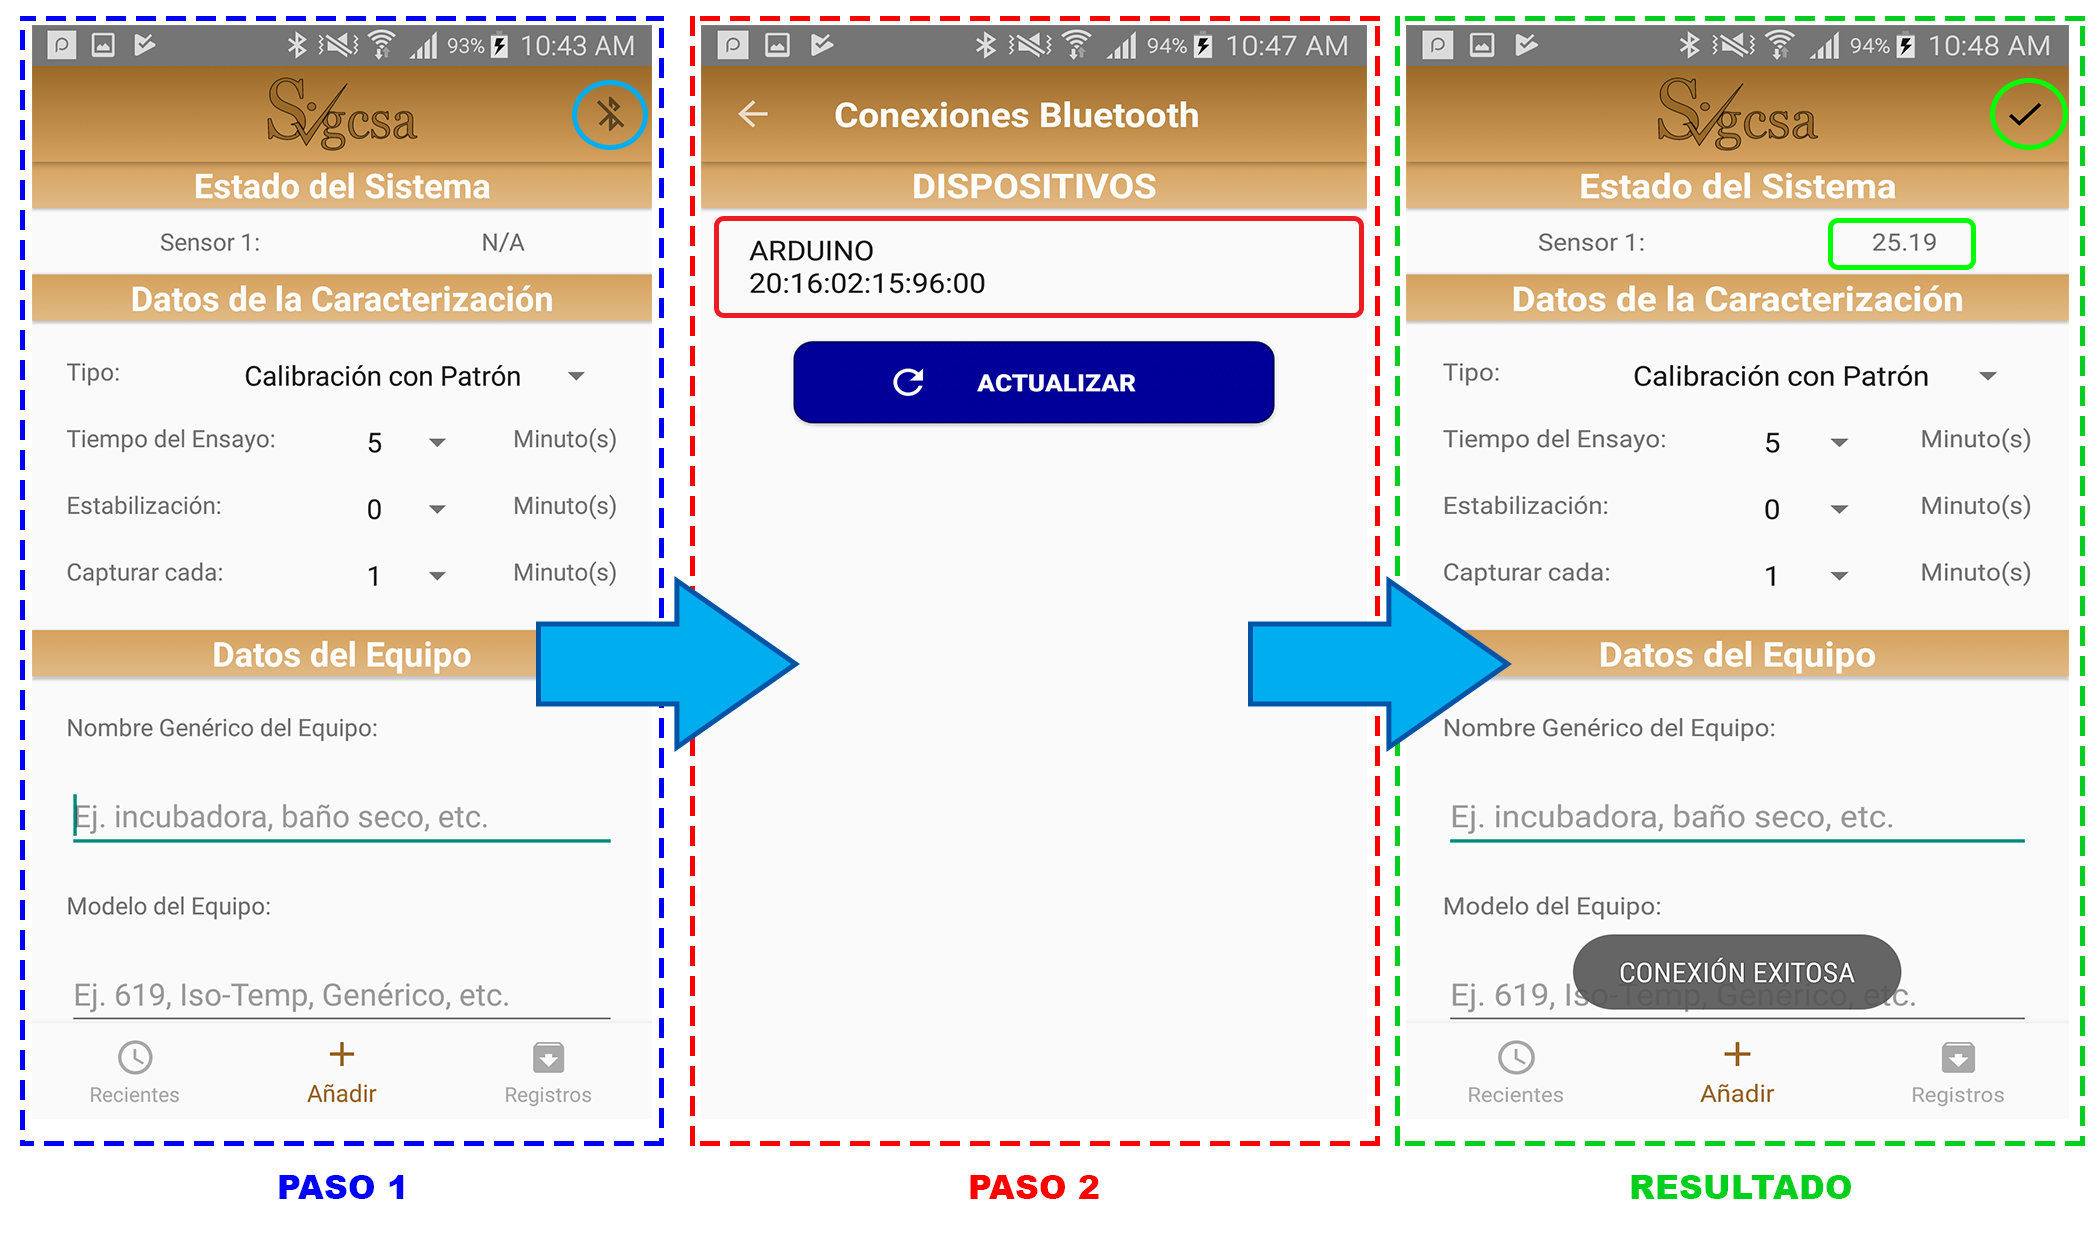
\includegraphics[width=0.8\linewidth]{interfaz13.png}
	\caption{Pasos para establecer conexión con el prototipo}
\end{figure}

\par \noindent
Si se realizó la conexión con el prototipo y la conexión se pierde se enviará un mensaje al usuario indicando lo sucedido.

\begin{figure}[H]
	\centering
	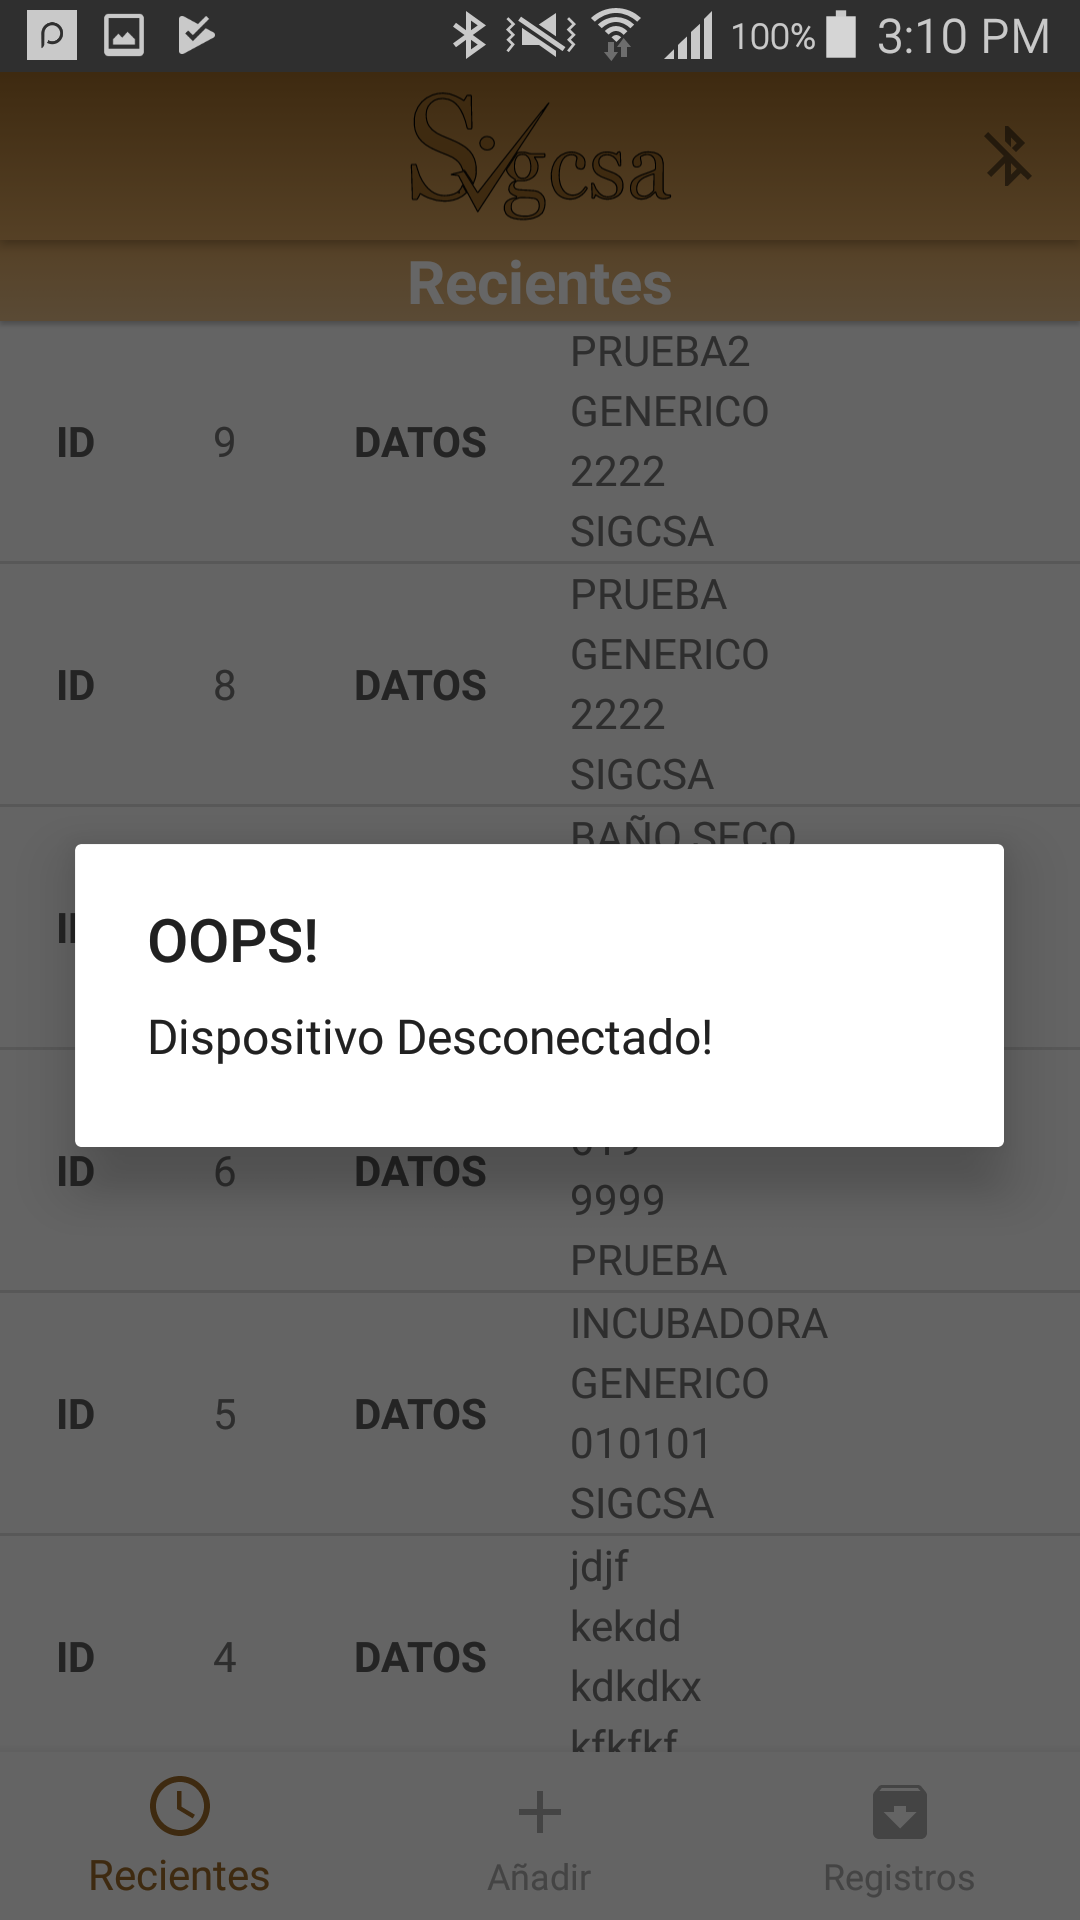
\includegraphics[width=0.3\linewidth]{interfaz14.png}
	\caption{Mensaje enviado al usuario por perdida de conexión con el prototipo}
\end{figure}

\par \noindent
Una vez establecida una conexión con el arquetipo se puede agregar un nuevo ensayo o medición.

\subsubsection{Agregar Nuevas Mediciones}

\par 
Primero hay que ubicarse en el fragmento añadir, menú inferior de la actividad principal botón "Añadir", la aplicación debe verse como en la imagen 3.14. se selecciona el tipo de ensayo, el tiempo del mismo, el tiempo de estabilización y el tiempo de captura. Luego se encuentran campos de texto para ingresar los datos del equipo a realizar el ensayo, estos campos son de texto libre. Si se llenaron todos los campos de texto y hay una comunicación activa con el dispositivo, el botón "INICIAR ENSAYO" se habilitará y cambiará a un color verde. Si se llenarón los campos de texto; pero, no hay una conexión activa con el prototipo o viceversa, el botón "INICIAR ENSAYO" no se habilitará.

\begin{figure}[H]
	\centering
	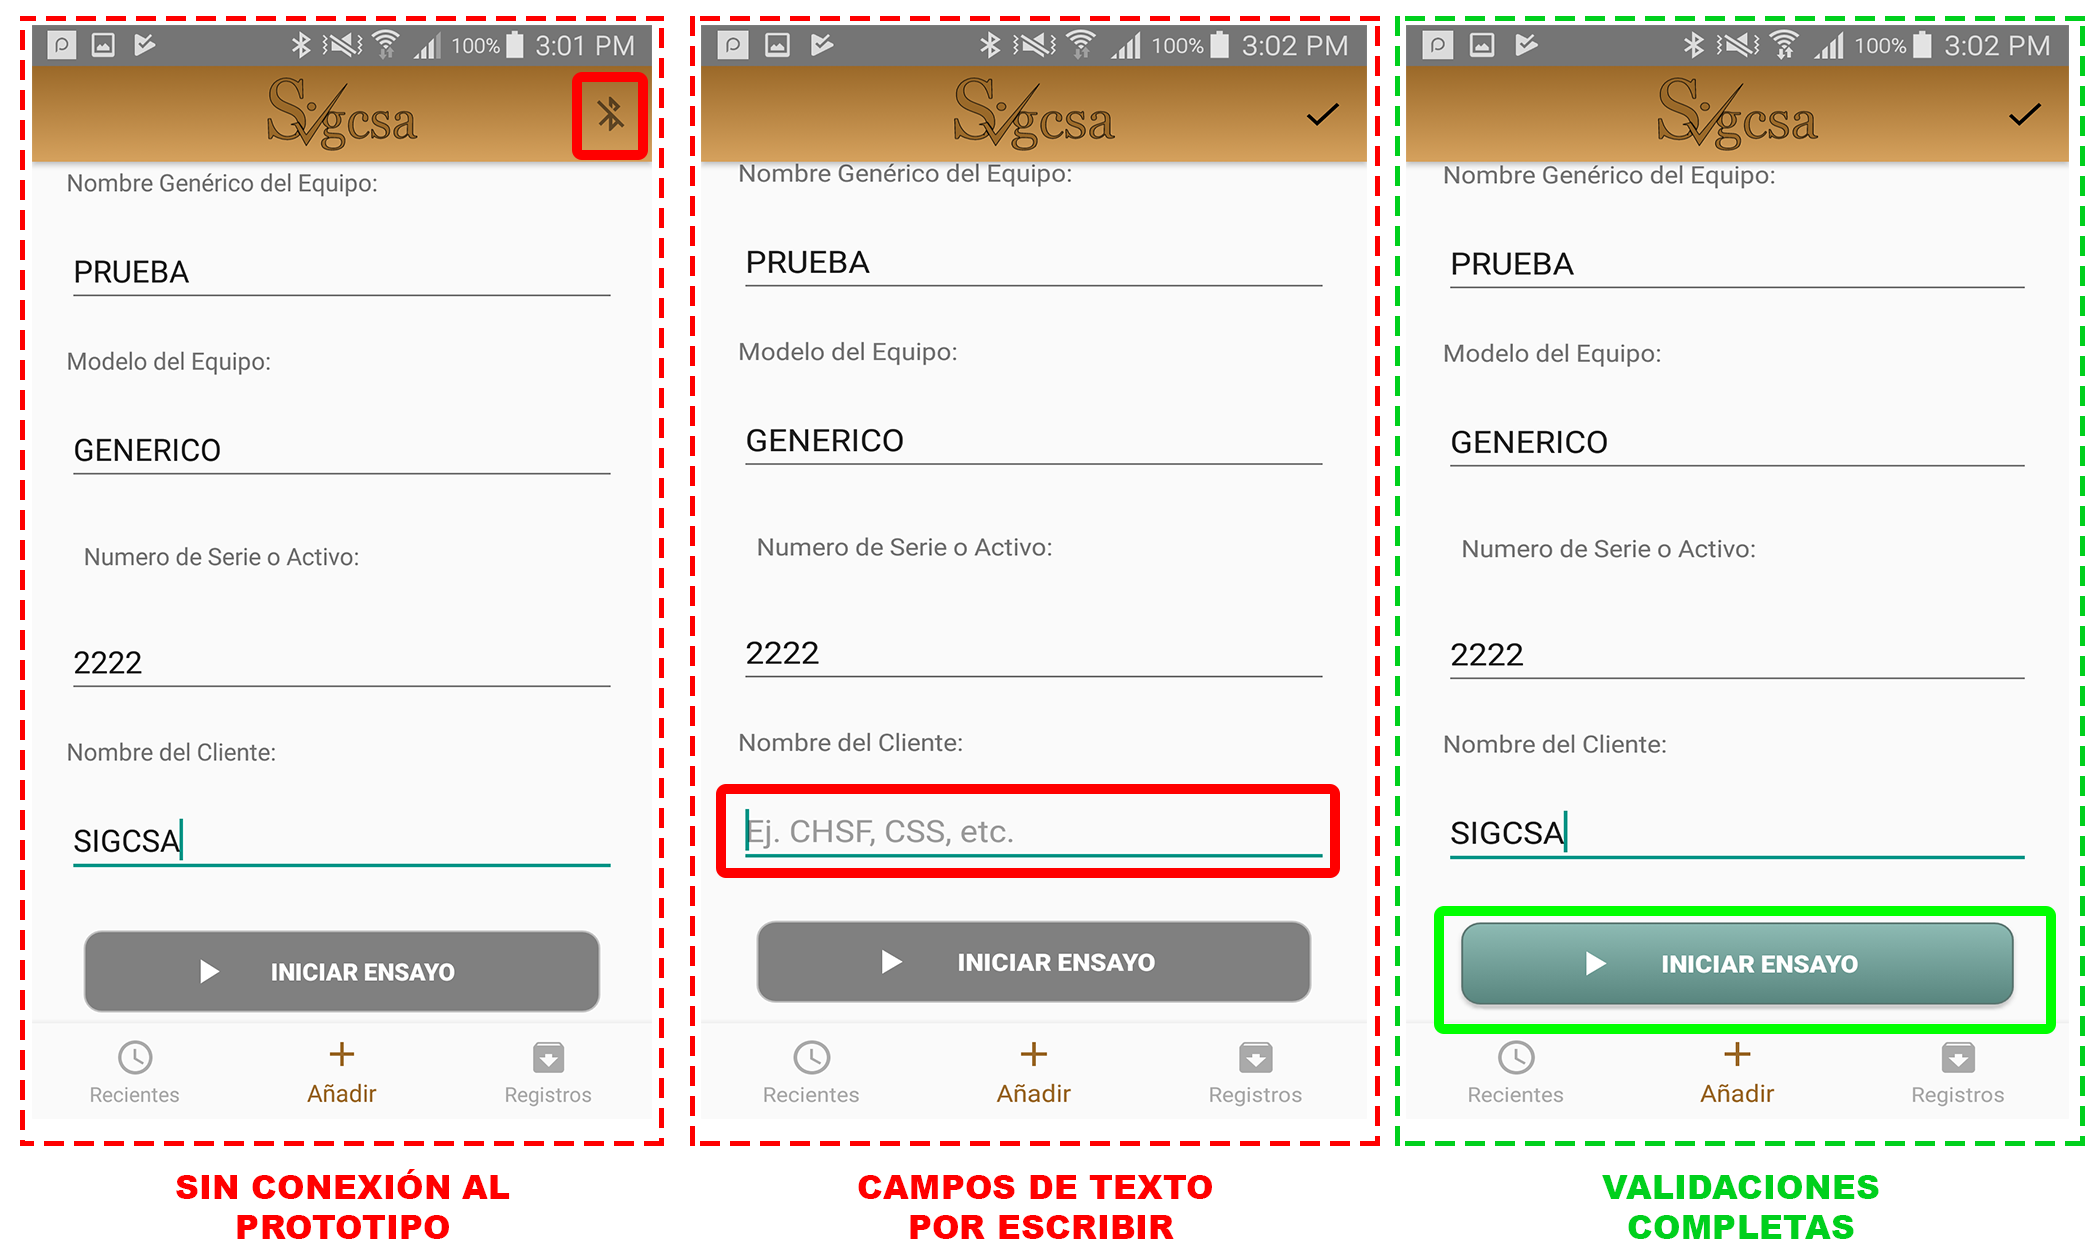
\includegraphics[width=\linewidth]{interfaz15.png}
	\caption{Validación Antes de Iniciar un Nuevo Ensayo}
\end{figure}

\par \noindent 
Una vez pulsado el botón "INICIAR ENSAYO", se deshabilitará el boton en cuestión y se habilitará el botón "CANCELAR". Además los parámetros de la medición se deshabilitarán para evitar cambios. Lo más importante es que inicia el servicio registros de mediciones el cual es el encargado de capturar los valores de los prototipos e insertarlos en la base de datos de la aplicación siguiendo los parámetros establecidos al inicio. 

\begin{figure}[H]
	\centering
	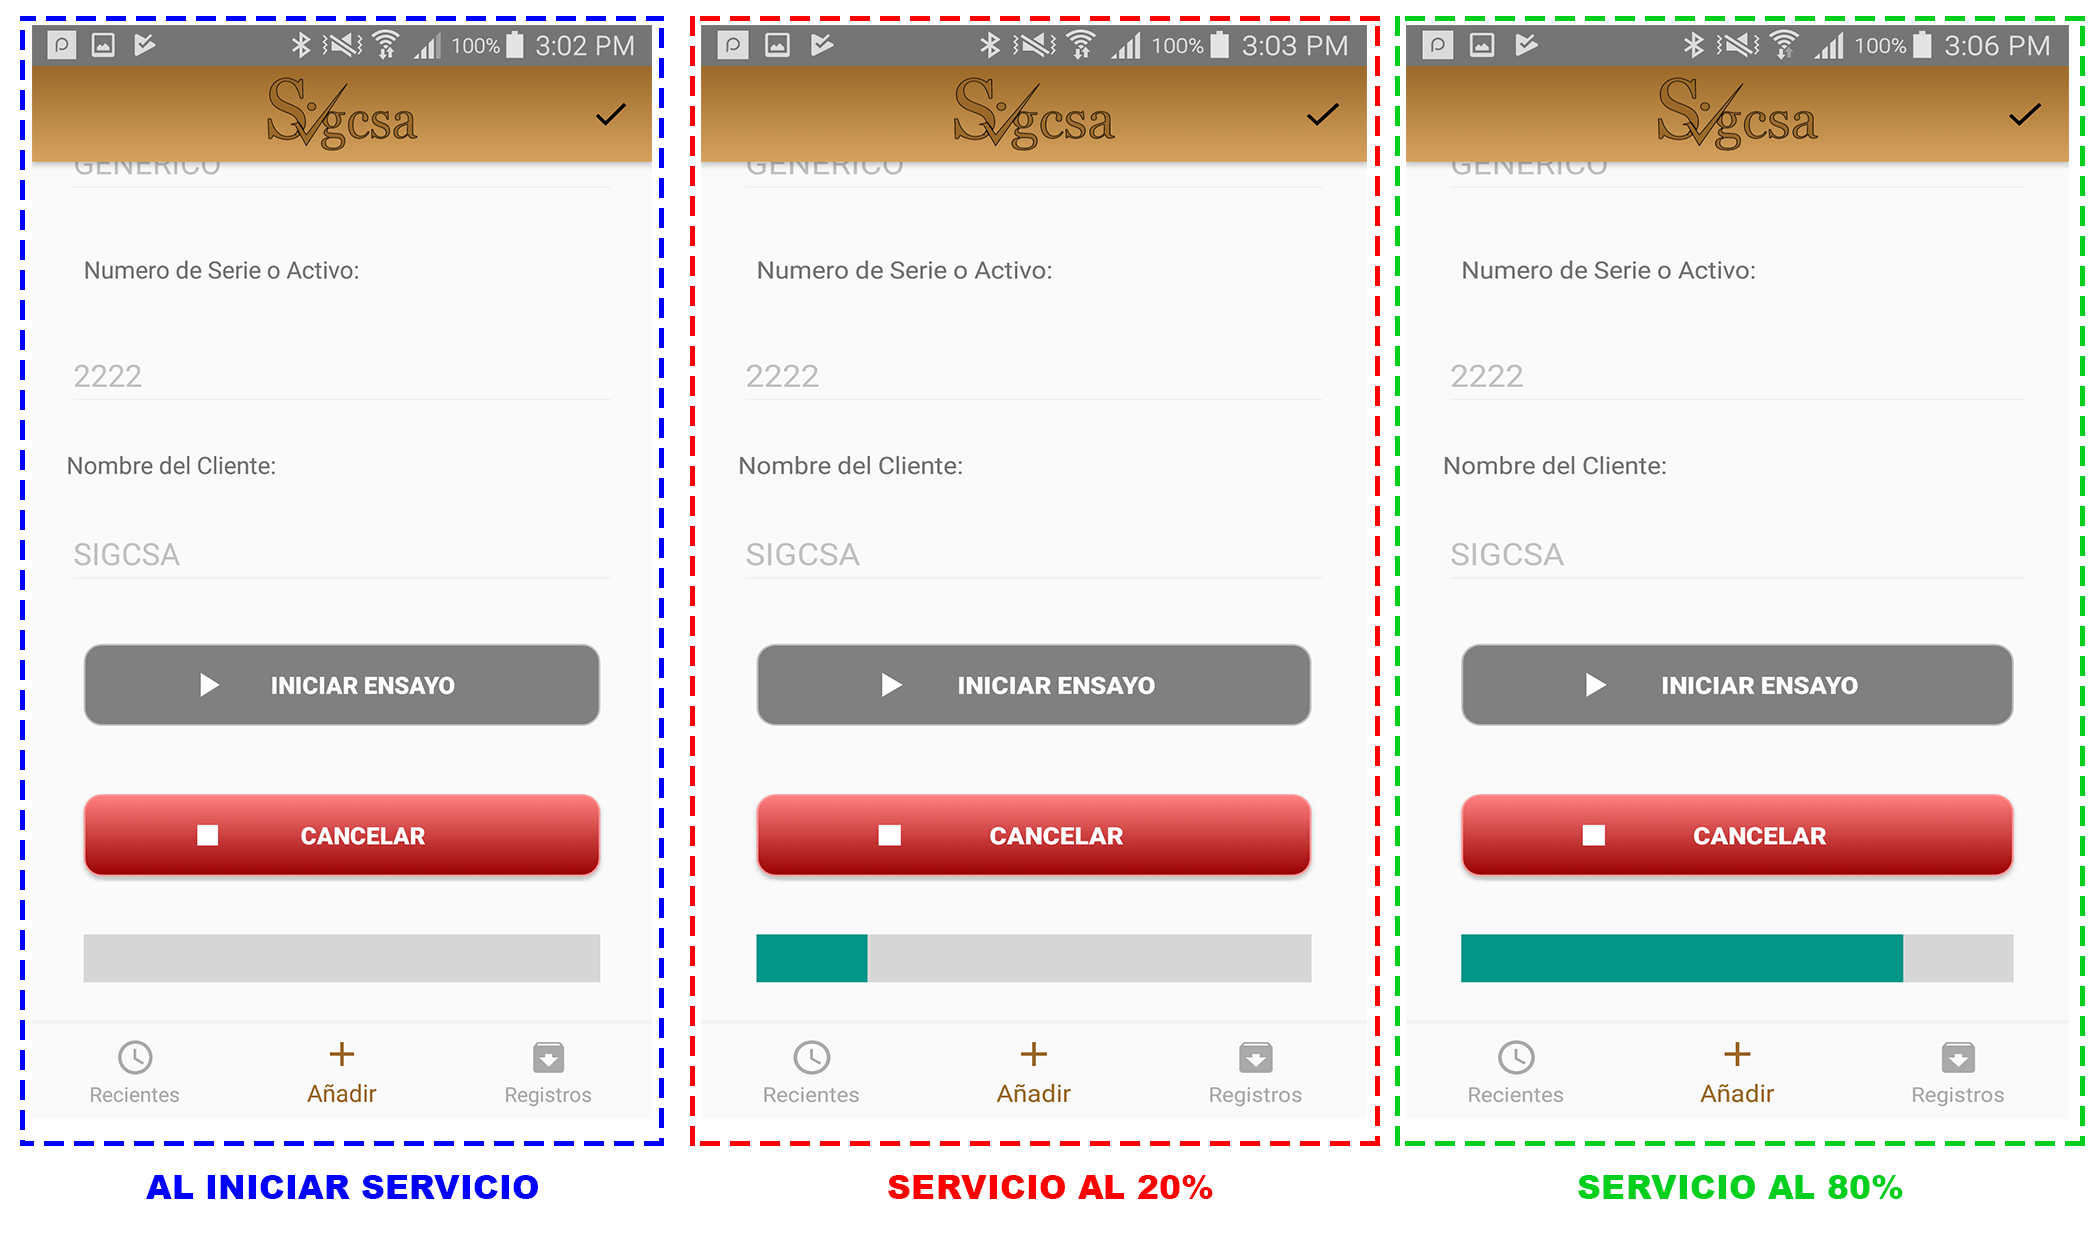
\includegraphics[width=\linewidth]{interfaz16.png}
	\caption{Proceso una vez pulsado el botón "INICIAR ENSAYO"}
\end{figure}
 
\par \noindent
Si el botón "CANCELAR" es pulsado es enviado un mensaje al servicio registros de mediciones para detener el proceso. Los valores como campos de texto y selecciones se vuelven a habilitar y el "progressbar" es reiniciado. Pulsado el botón "INICIAR SERVICIO" automáticamente se graba una fila en la base de datos. Si el servicio finaliza correctamente los valores de los campos de texto se limpian y queda el ingresa en la base de datos como "COMPLETADO". 

\par \noindent
Otro punto importante es que como el servicio registro de mediciones y servicio bluetooth de la aplicación se ejecutan en segundo plano esto quiere decir que mientras la aplicación no sea borrada de memoria. Se puede ir a otra aplicación como por ejemplo: WhatsApp, Correo, YouTube, etc. y el programa se seguirá ejecutando. Para uno se ejecutará según desee el usuario 5 minutos o una hora; mientras que, el otro se ejecuta hasta que se pierda conexión del prototipo o que se deshabilite el bluetooth del teléfono.

\par \noindent
Una vez ejecutado un ensayo hay que asegurarse que la base de datos se haya actualizado correctamente; para poder consultar las mediciones de temperatura después.

\subsubsection{Consultar una Medición Realizada Recientemente}

\par 
Para consultar una medición realizada recientemente basta solo con ubicarse en la actividad principal y seleccionar el botón "Recientes". Cada vez que se regrese al fragmento recientes, se consulta a la base de datos de la aplicación y se retornan los últimas 10 mediciones o ensayos realizados. La aplicación debe verse como en la imagen 3.11 donde se encuentra una lista de mediciones cada una con su respectiva información y número de registro (ID). Al seleccionar un elemento de la lista se desplegará más información de la medición como en la imagen 3.19. En ella se puede acceder a las mediciones de temperatura de cada sonda de manera individual con sus respectivas características como en la imagen 3.20.

\begin{figure}[H]
	\centering
	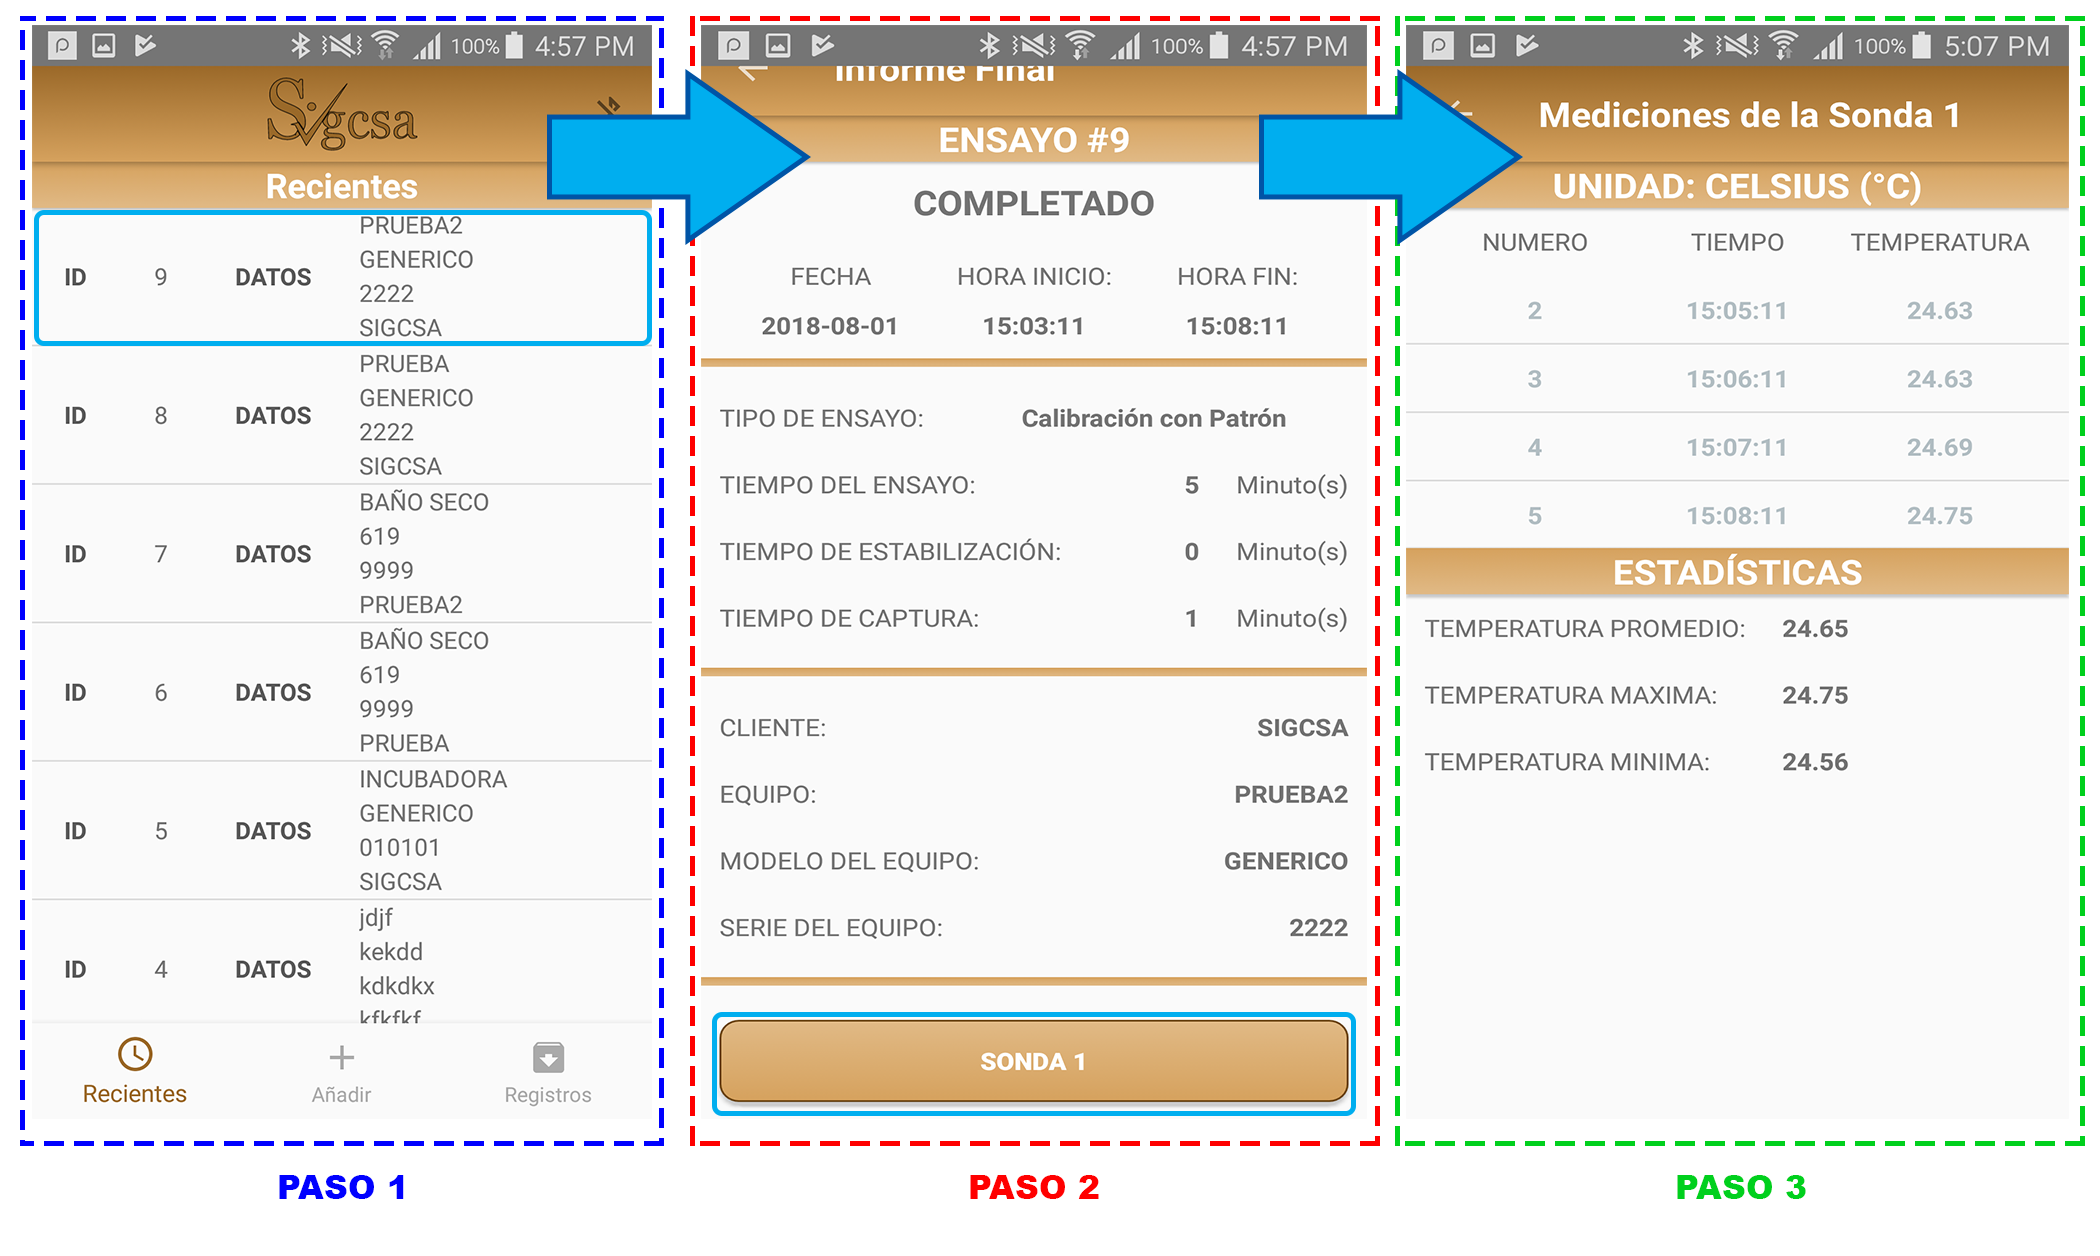
\includegraphics[width=\linewidth]{interfaz17.png}
	\caption{Proceso para consultar temperatura de una respectiva sonda en un ensayo}
\end{figure}

\par \noindent
Siempre es posible regresar al paso anterior utilizando el botón en la esquina superior izquierda o presionando la tecla de regreso del teléfono. Por último como se consulta un ensayo en un intervalo de fechas predeterminadas. 

\clearpage

\subsubsection{Consultar una Medición Realizada en una Fecha Específica}

\par 
Para consultar una medición o ensayo de una fecha específica o en un intervalo de fecha solamente hay que ubicarse en el fragmento registros, actividad principal seleccionar botón registros. La aplicación debe verse como en la imagen 3.16. Se seleciona uno de los campos con el texto "N/A" y se eligen las fechas deseadas, uno es para la fecha inicio la otra es para la fecha fin y se presiona el botón buscar. De encontrarse resultados se desplegarán en un formato de lista idéntico al formato del fragmento recientes y el proceso para consultar la información es igual al proceso anterior.

\begin{figure}[H]
	\centering
	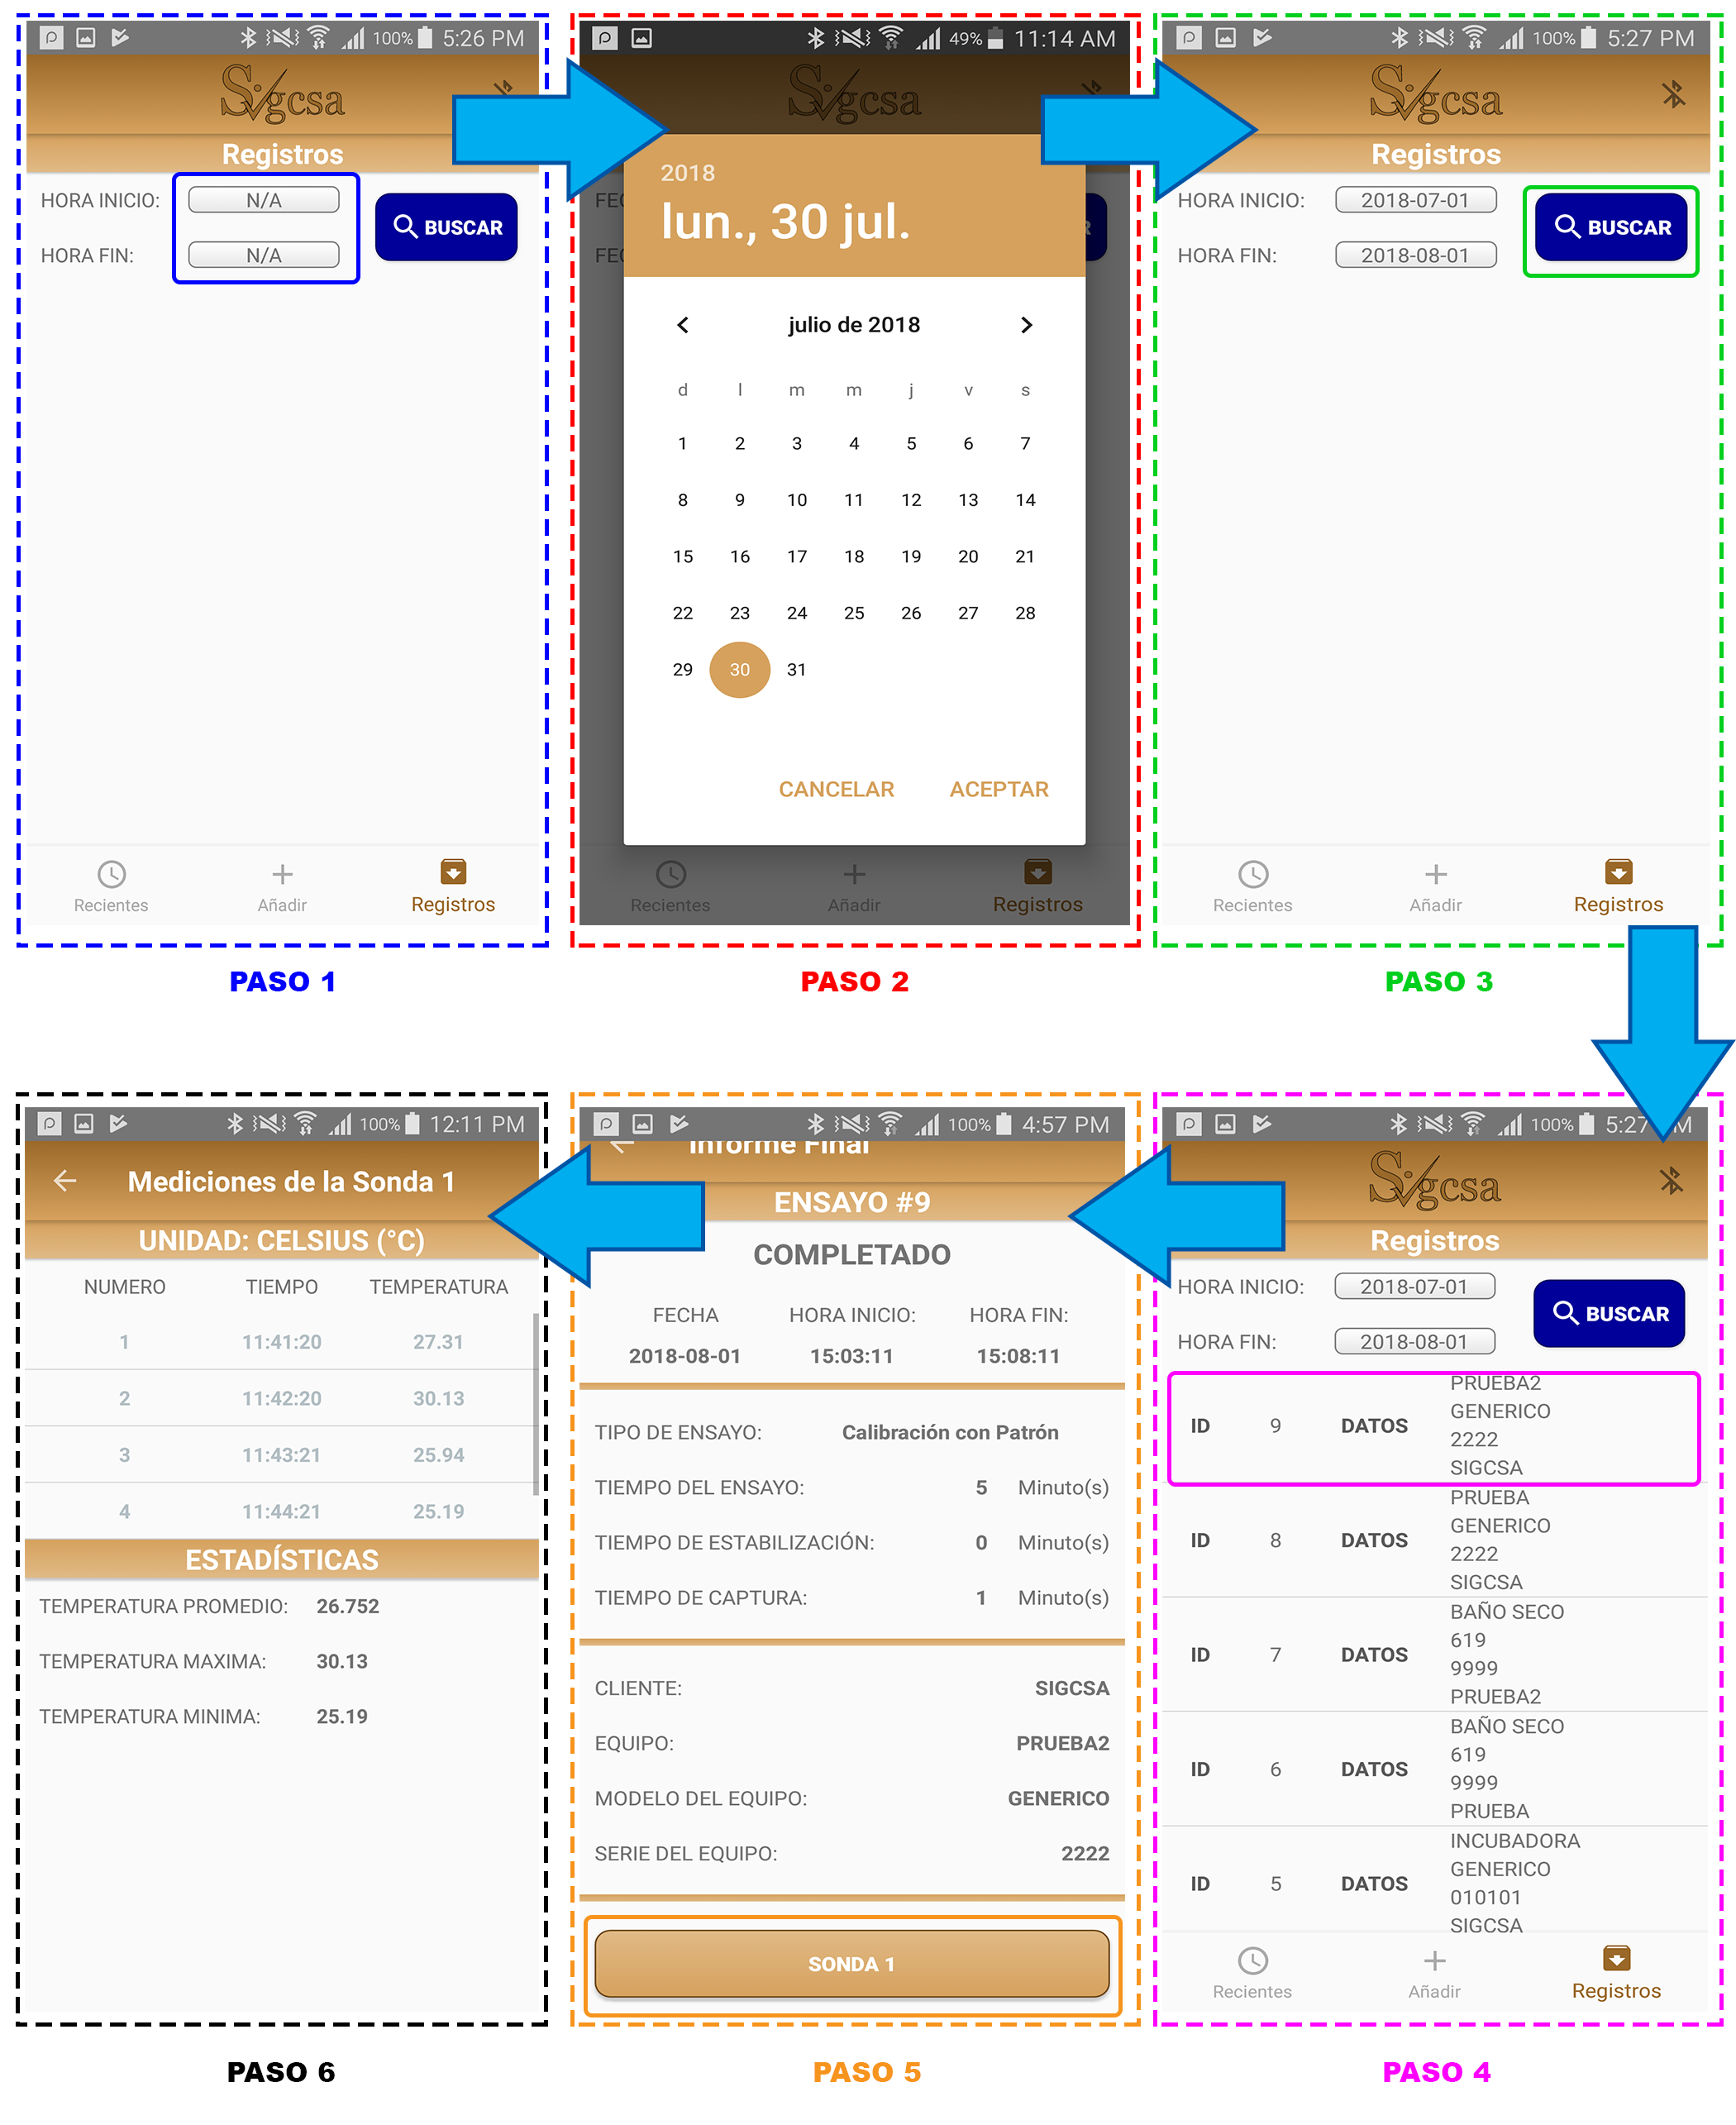
\includegraphics[width=0.8\linewidth]{interfaz18.png}
	\caption{Proceso para consultar temperatura de una respectiva sonda en un ensayo en un intervalo de fechas}
\end{figure}

\par \noindent
Se tiene conocimiento de las interfaces que se encuentran en la aplicación y como utilizarlas; sin embargo, no se sabe la parte técnica. Cuando se presionan ciertos botones se hacen llamadas a servicios que se ejecutaran en el segundo plano pero ¿Como funcionan estos servicios?
